\section{Implementation}
\subsection{Sweep Line Segment Intersection}
The line segment intersection algorithm is implemented following the Bentley-Ottmann algorithm described in the section above.

For the data structures, the implementation uses a Red-Black Tree as the event queue where the events are sorted based on descending y-coordinate and ascending x-coordinate. This is equivalent to having a sweep line moving from top to bottom and from left to right in case of events with the same y-coordinate.

For the status structure, a simple list was used to store the segments that are currently intersecting the sweep line. The list is sorted based on the x-coordinate of the intersection point with the sweep line. Initially, the status structure was implemented using a Red-Black Tree as well but updating the position of the segments every time the sweep line moved proved to be too complex. Moreover, the number of segments in the status structure is expected to be small, so the performance loss is only visible in worst case scenarios where a large number of segments all intersect the sweep line at the same time.

As a result, the overall complexity of the algorithm is worse than the theoretical complexity of $O(n\log n + k \log n)$, where $n$ is the number of segments and $k$ is the number of intersections. The complexity of the implementation is $O(n\log n + k n\log n) = O(kn\log n)$ because keeping the status structure sorted requires $O(n\log n)$ instead of $=O(\log n)$ for a balanced search tree.

Another aspect that needed careful consideration was the handling of degenerate cases:
\begin{itemize}
    \item \textbf{Horizontal Segments}:  Horizontal segments are handled by sorting the events based on the x-coordinate of the left endpoint of the segment. This ensures that the left endpoint is always processed before the right endpoint.
    \item \textbf{Colinear Segments}: Colinear segments are considered as intersecting at the endpoints. This requires special handling because differently from all other cases, the intersection point is not unique . The implementation manually adds the intersection points instead of relying on the algorithm to compute them.
\end{itemize}


Below we can compare the performance of the sweep line intersection algorithm and the naive algorithm. It is interesting to notice how in the comparison based on the number of intersections, the naive algorithm can sometimes outperform the sweep line approach. This is due to the fact that the naive algorithm is not affected by the number of intersections but only by the number of input segments.
\begin{figure}[H]
    \begin{subfigure}{0.5\textwidth}
        \centering
        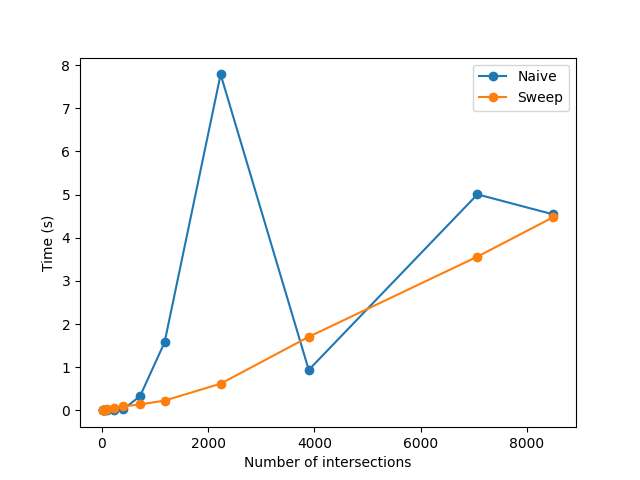
\includegraphics[width=\linewidth]{images/plot_intersections.png}
        \caption{Comparison based on the number of intersections}
        \label{fig:intersections}
    \end{subfigure}
    \begin{subfigure}{0.5\textwidth}
        \centering
        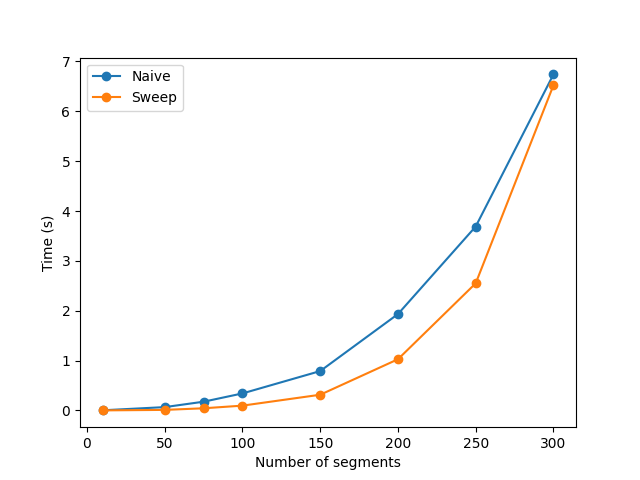
\includegraphics[width=\linewidth]{images/plot_segments.png}
        \caption{Comparison based on the number of segments}
        \label{fig:segments}
    \end{subfigure}
\end{figure}


\subsection{Overlay of Two Subdivisions}
The first step for the implementation of the overlay algorithm is the construction of the Doubly Connected Edge Lists. Since the implementation was done in Python, keeping track of pointers between the different elements isn't as straightforward as in other lower-level languages. To overcome this, the implementation uses a series of dictionaries to store vertices, half-edges and faces while each element only contains the unique identifies. This way, the pointers are replaced by the identifiers and the dictionaries can be used to access the elements on $O(1)$ time. Compared to storing the entire object, this approach is more memory efficient and less prone to errors because a single copy of the object is stored in memory.

\begin{minipage}{0.5\linewidth}
    \begin{lstlisting}
class Vertex:
    id: VertexId
    coordinates: Point
    incident_edges: List[EdgeId]
\end{lstlisting}
\end{minipage}
\begin{minipage}{0.5\linewidth}
    \begin{lstlisting}
class Edge:
    id: EdgeId
    origin: VertexId
    twin: EdgeId
    incident_face: FaceId
    next: EdgeId
    prev: EdgeId
\end{lstlisting}
\end{minipage}

\begin{minipage}{\linewidth}
    \begin{lstlisting}
class Face:
    id: FaceId
    outer_component: EdgeId
    inner_components: List[EdgeId]
    area: float
    info: str
\end{lstlisting}
\end{minipage}

Take for example the \texttt{Edge} class. The class contains its unique identifier, the identifier of the origin vertex, the edge ids of its twin, next and previous edges and the identifiers of the face it belongs to. If instead of storing the identifiers, the class stored the actual objects (e.g. \texttt{Vertex} instead of \texttt{VertexId}), the memory usage would be higher because each object would contain a copy of the other objects it references. Moreover, the implementation would be more error-prone because changing an object would require updating all the references to it.

Some differences with respect to the theoretical data structure are present:
\begin{itemize}
    \item \textbf{Vertex}: each vertex stores a list of incident edges instead of a single edge. This is not strictly necessary but it simplifies the implementation because it allows to easily access and update the edges incident to a vertex and this is done often during the overlay algorithm.
    \item \textbf{Face}: each face stores the area of the face and an info string in addition to the standard fields. The signed area is computed as follows
          \begin{equation*}
              A = \frac{1}{2} \sum_{i=0}^{n-1} (x_i y_{i+1} - x_{i+1} y_i)
          \end{equation*}
          and is used during the DCEL construction to determine the unbounded face: faces with a negative area are considered unbounded.

          The info string is used to optionally store information about the face. In the final overlay, the info field is used to store the input subdivisions that intersect in the face.
\end{itemize}

The overlay algorithm is implemented similarly to how its was described in the theoretical section with the major difference being that the overlay isn't computed during the sweep line algorithm but after. This allows to keep the two step separate and more easily debug the algorithm without increasing the overall complexity. The only additional computation in the sweep line algorithm is keeping track of each segment and in how many points it is intersected by other segments. This information is then for two purposes:
\begin{itemize}
    \item To split edges at the intersection points. This is particularly useful when an edge is intersected multiple times by the other subdivision.
          \hfill \break
          \begin{minipage}{0.7\linewidth}
              For example, the edge $e$ is intersected in two points. The edge is first split at the first intersection point and divided in $e_1^{\prime}$ and $e_1^{\prime\prime}$; $e_1^{\prime\prime}$ then has to be split again at the second intersection point to obtain $e_2^{\prime}$ and $e_2^{\prime\prime}$. Instead, if we already know that $e$ is intersected in two points, we can directly construct only $e_1^{\prime}$, $e_2^{\prime}$ and $e_2^{\prime\prime}$.
          \end{minipage}
          \begin{minipage}{0.3\linewidth}
              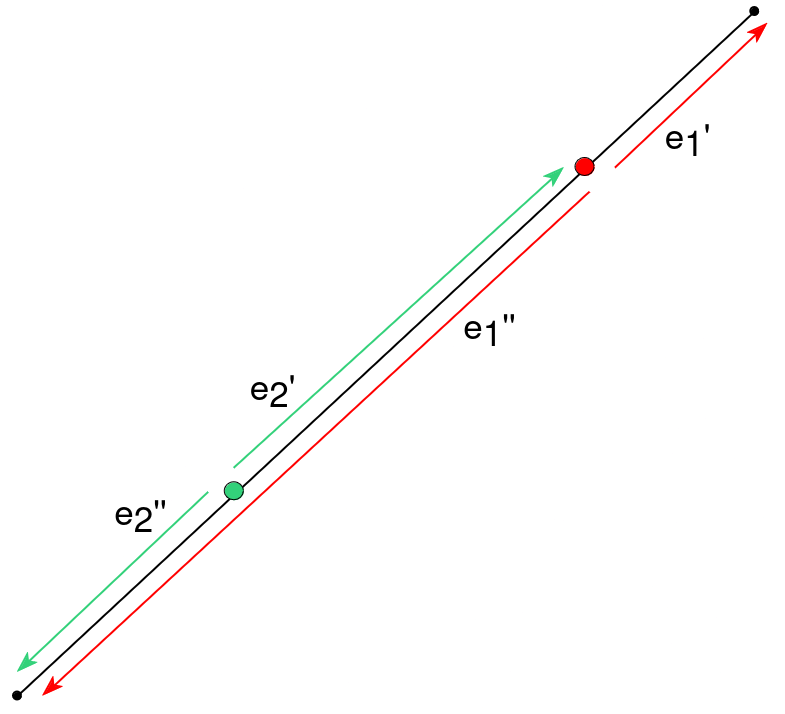
\includegraphics[width=\linewidth]{images/split.png}
          \end{minipage}
    \item To determine the faces from the original subdivisions that make up a face in the overlay: for each split edge that is now part of a specific face in the overlay, we know the original edge it was a part of and the face it belonged to.
\end{itemize}

Below we can see an example of the overlay algorithm applied to two simple subdivisions
\begin{figure}[H]
    \begin{subfigure}{0.5\textwidth}
        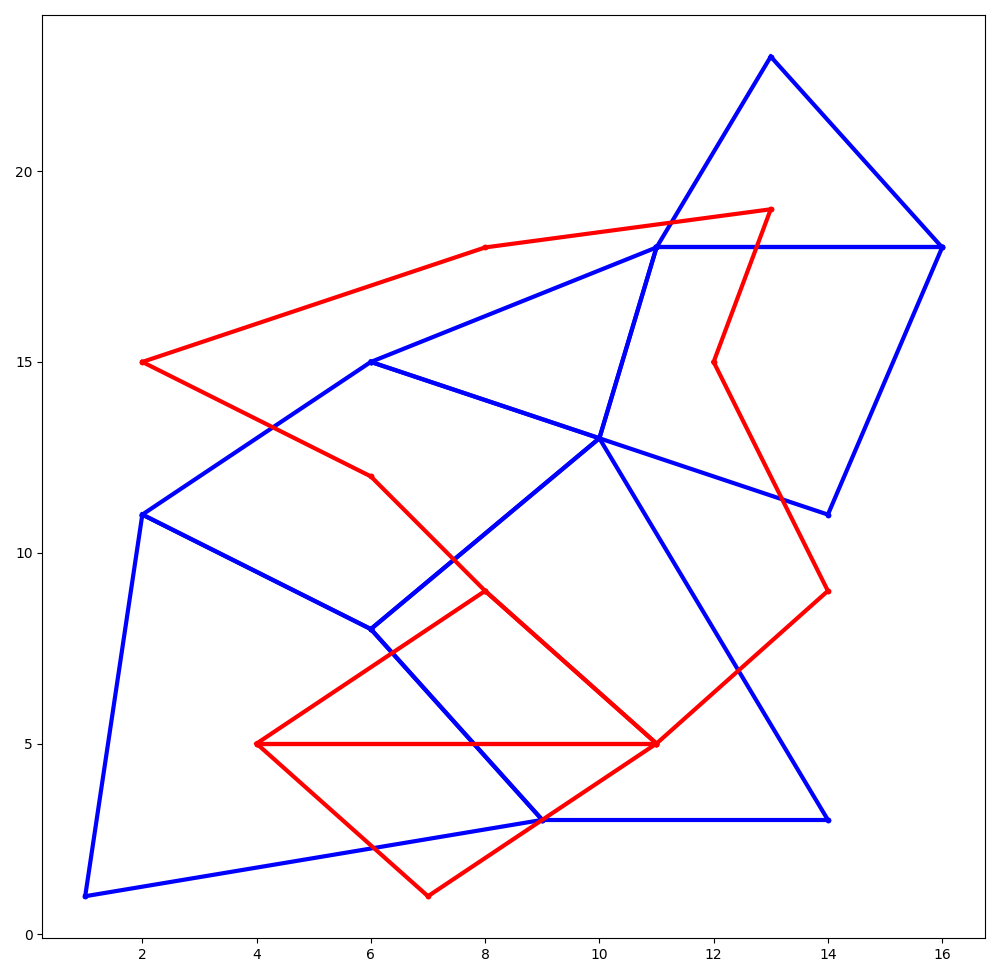
\includegraphics[width=\linewidth]{images/test_1_test_2_dcels.png}
        \caption{Original subdivisions}
        \label{fig:overlay_subdivisions}
    \end{subfigure}
    \begin{subfigure}{0.5\textwidth}
        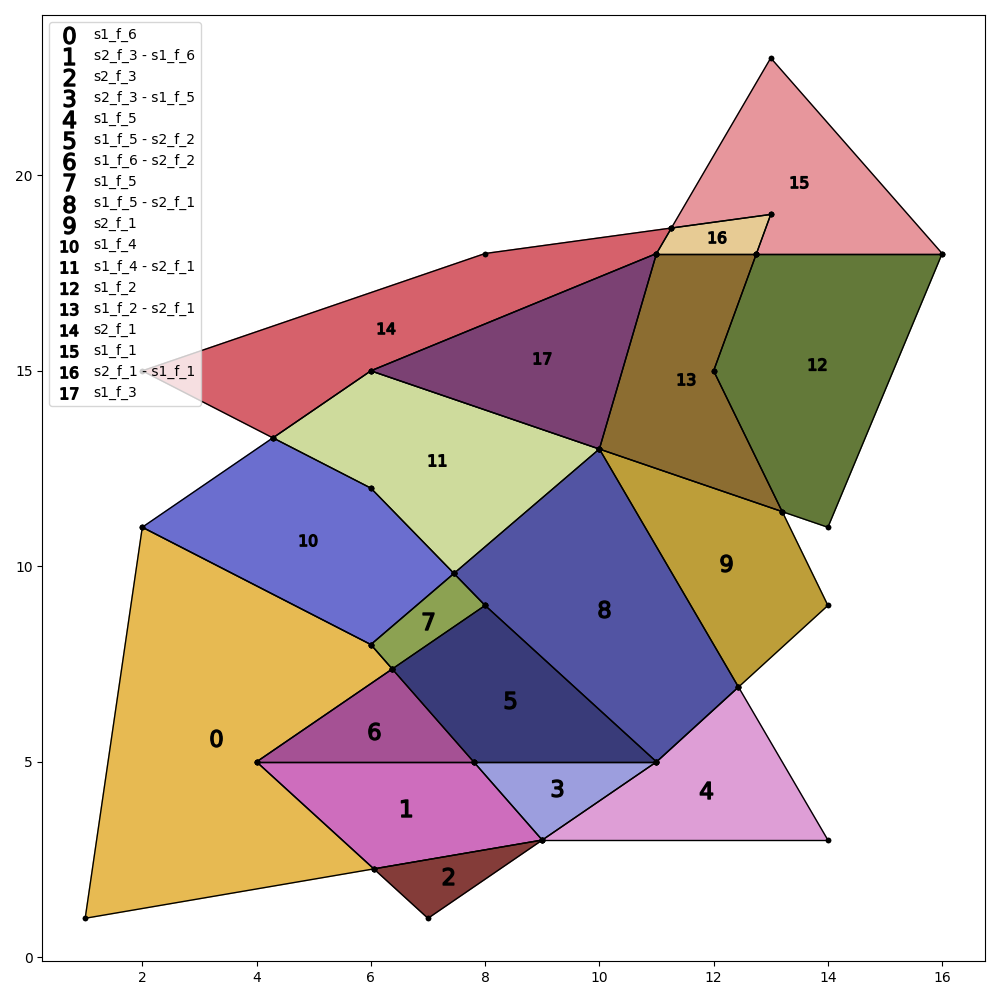
\includegraphics[width=\linewidth]{images/test_1_test_2.png}
        \caption{Overlay of the two subdivisions}
        \label{fig:overlay_result}
    \end{subfigure}\\
    \break
    \begin{subfigure}{\textwidth}
        \centering
        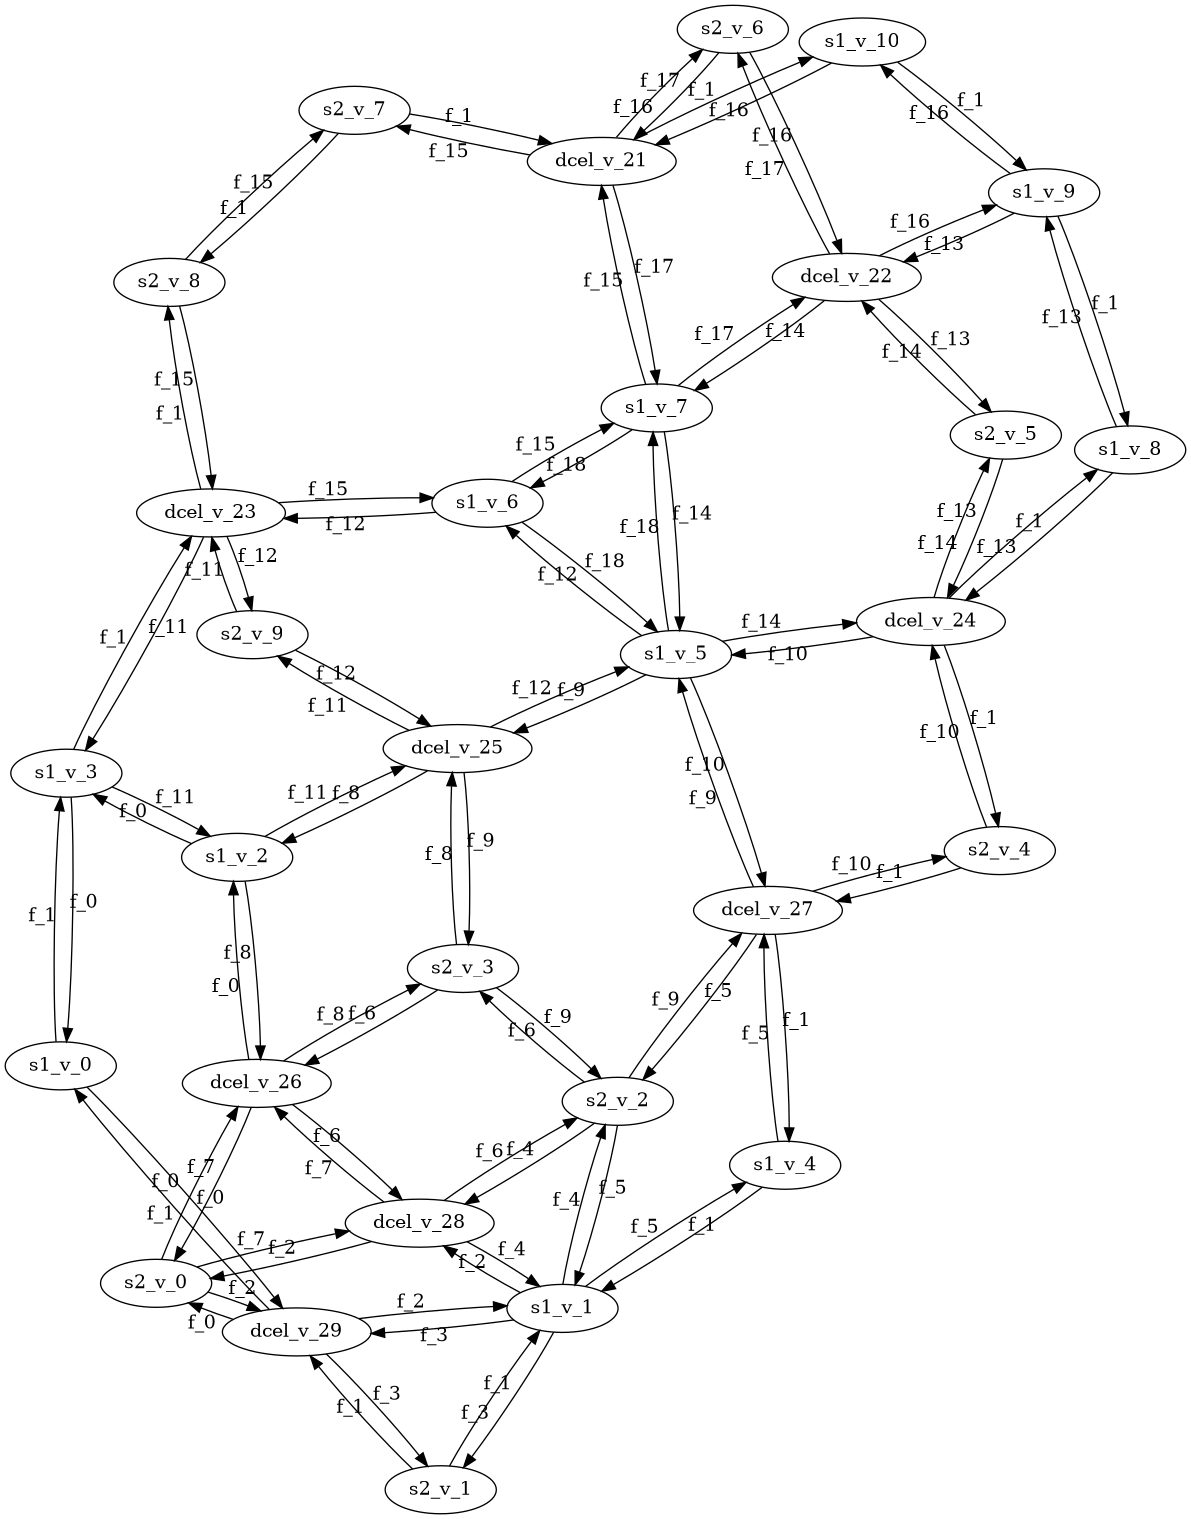
\includegraphics[width=0.5\linewidth]{images/test_1_test_2_graph.png}
        \caption{Different representation of the overlay}
        \label{fig:overlay_faces}
    \end{subfigure}
\end{figure}

Similarly to the theoretical description, the overlay algorithm doesn't increase the complexity with respect to the line segment intersection algorithm but, given the suboptimal complexity of our intersection algorithm implementation, the overall complexity is $O(kn\log n)$ where $n = n_1 + n_2$ is the total number of segments in the two subdivisions and $k$ is the number of intersections.
